This section describes our system architecture.
An overview over the architecture is shown in figure \ref{fig:architecture}.
\begin{figure}[!h]
	\centering
		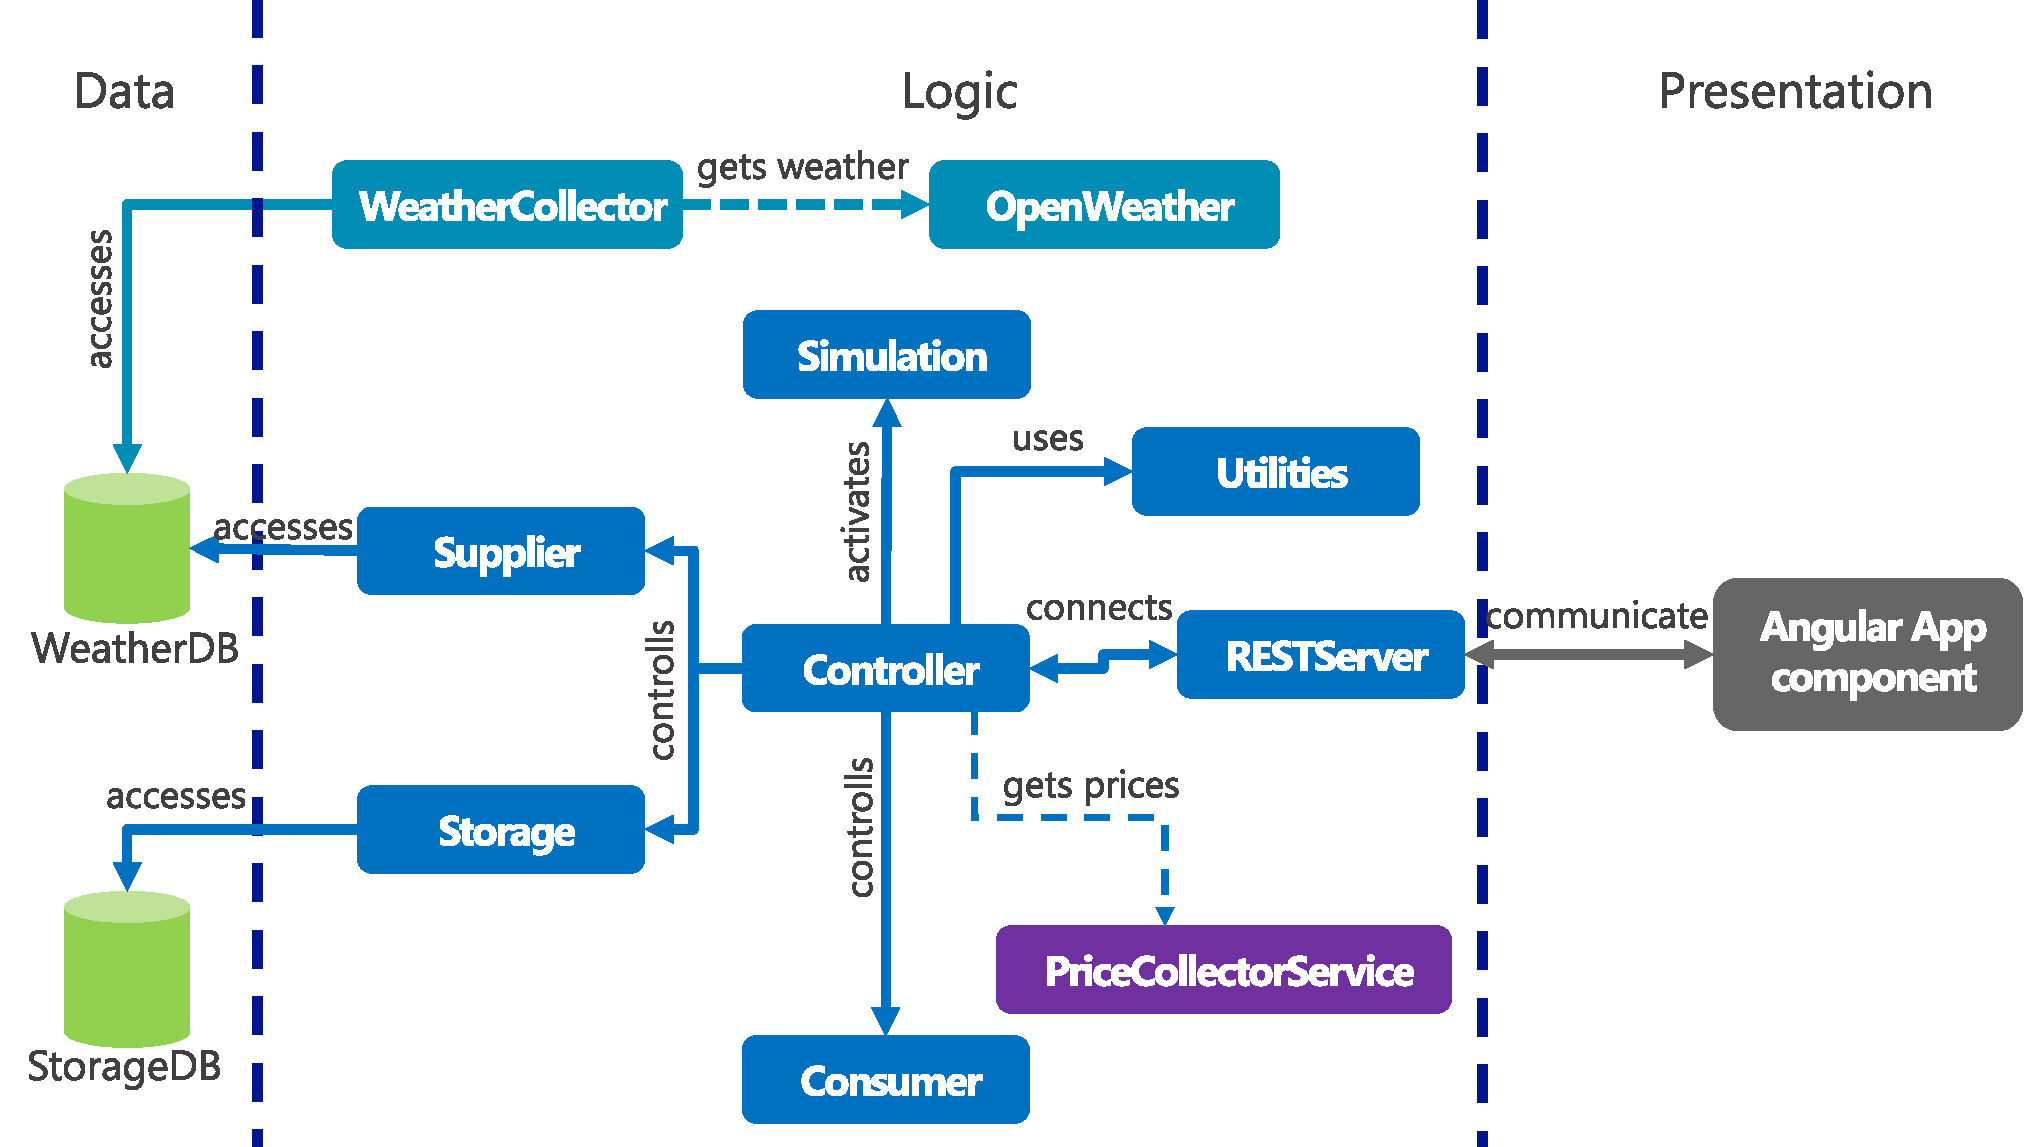
\includegraphics[width=1.00\textwidth]{../figures/Architecture.pdf}
	\caption{Smart energy system architecture}
	\label{fig:architecture}
\end{figure}

The \texttt{WeatherCollector} component is responsible for gathering actual weather data from \textit{OpenWeather} API.
This weather data is stored into a database for further use of the supply and demand components of the system.

In order for the whole system to be reliable and responsive we separated the \texttt{WeatherCollector} component from the rest of the system.
It speaks only to the weather database where it get the locations for which it should collect weather data.
The collected data gets written into the database and stored.
Even in the case of a failure of the weather component or OpenWeather the already collected data is still accessible and therefore the system can work with it, making the system independent of the weather component.
In the case of a new registration of a supplier component during a weather component failure, the database may return default values for the new component in a way the running system is not being halted by missing data.
These measures should make the system reliable and and responsive in that context.\\
\\
The three-layered architecture was already planned for in the first conceptions of the project, therefore no extra steps had to be taken.
We divided the project in subcomponents and put them in the respective part of the architecture.\\
The first layer is the data layer which only consists of data-providing hardware and databases. 
Since the current project does not include data-providing hardware (as far as the current conception goes) only databases are left in this layer.\\
The second layer consists of the functional components of the project.
All suppliers, storages, consumers and utility components are part of this layer, since they mostly take data from the databases and compute their respective power in- and output based on those values and give them to the simulation component.
The simulation component is part of this layer, and takes the data the other component in order to model the different interactions of the smart grid.
The workflow is controlled by the controller component and connects all components together.
The last component in this layer is the REST component which makes the computed data from the simulation component available to the frontend layer.\\
The frontend layer is the third and last layer in our project.
It handles the interaction with the user and makes it possible for the user to add and remove components to the smart grid simulation as he sees fit.